\section{\sys{}: a staged investigation}
\label{sec:agent}

\begin{figure*}[t]
\centering
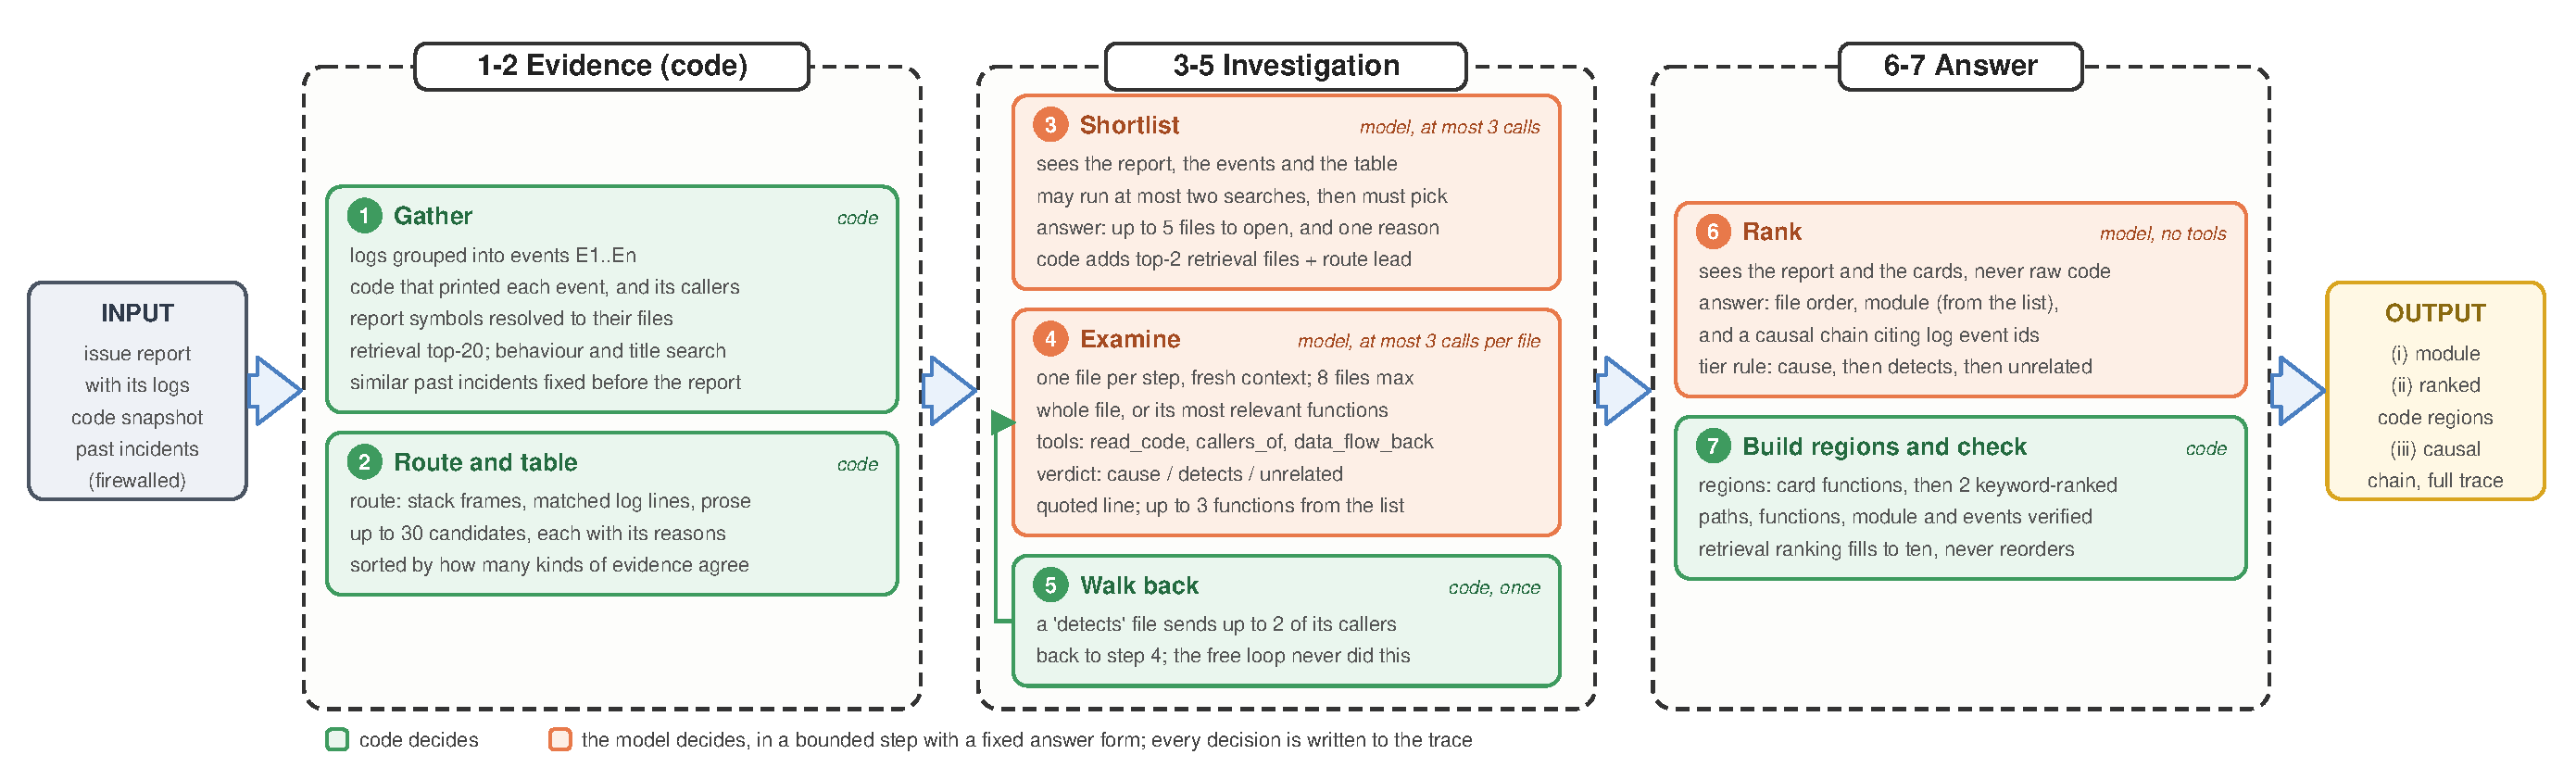
\includegraphics[width=0.98\textwidth]{figures/workflow.pdf}
\caption{\sys{}. Code gathers the evidence and builds a candidate table
(1, 2). The model then makes three kinds of decision, each in a bounded
step with a fixed answer form: which files to open (3), what role one
file plays (4, one file per step, the code on screen), and the order of
the files (6, from the verdict cards only). Code walks back from files
that only detect the failure (5) and checks the answer (7). Green steps
are code; orange steps are the model.}
\label{fig:workflow}
\end{figure*}

\sys{} runs on one general-purpose 27B open-weights model, self-hosted,
at temperature zero with a fixed seed. Its inputs are the issue report
with its logs, the code snapshot, and the project's incident memory
behind the firewall of \cref{sec:approach:firewall}. Its outputs are
the affected module, a ranked list of code regions (file and
function), and a chain of steps from the reported
symptom to the named cause, each step citing a log event from the
report where one applies.

\subsection{Design principles}
\label{sec:agent:principles}

Localization agents are usually built as a loop: one model, a set of
tools, a turn budget, and the model deciding at every turn what to do
next and when to stop. \sys{} is built on four principles that take
those decisions away from the model. The evidence is gathered by code
before the model is called, so no turn is spent searching for what the
report already names. Every candidate file is judged on its own, in a
fresh context with its code on screen, so a file's rank depends on what
its code does rather than on how often or how recently it was read.
The step from a file that only detects a failure to the files that
could have caused it is taken by code, not left to the model. And the
run ends when the procedure ends, with a submission the schema requires
to be complete. What this structure is worth is measured in
\cref{sec:results:structure} against an ablation that gives the same
model the same tools in an unconstrained loop.

\subsection{The staged workflow}
\label{sec:agent:stages}

\Cref{fig:workflow} shows the procedure. It is fixed; the model decides
only inside it, three times, and every decision is written to the
trace.

\textbf{1. Gather (code).} Code collects the evidence before the model
is called. The logs in the report are grouped into events and labelled
\texttt{E1}, \texttt{E2}, \ldots; for each event the code finds the
statement that printed it and that statement's callers; every symbol in
the report is resolved to the file that defines it; the retrieval layer
of \cref{sec:approach} supplies its top twenty files; the incident
memory is queried, behind the firewall, for similar past incidents and
the files their fixes touched; a behaviour search and a title search run
over file content.

\textbf{2. Route and table (code).} The report is routed by what it
contains: stack frames, else log lines that match a statement in the
code, else prose. Every file any channel named goes into one candidate
table of up to thirty rows, each with the reasons it is there
(``declares \texttt{SequenceNumber}'', ``fixed in past incident
KAFKA-5342'', ``prints log event E2''). The table is sorted by how many
kinds of evidence point at a file.

\textbf{3. Shortlist (model, at most three calls).} The model sees the
compressed report, the events and the table, may run at most two
searches if the table clearly misses the described behaviour, and must
answer with up to five paths to examine. Code keeps only paths that are
in the table or that the model's own searches returned, and always adds
the top two retrieval files and the route's lead file, whether or not
the model picked them.

\textbf{4. Examine (model, one file per step, at most three calls
each).} Each queued file is judged alone, in a fresh context that holds
only the report and that file: the whole file when it fits 24{,}000
characters, otherwise its most relevant functions whole, most relevant
first, until the budget is full, plus the list of every function the
file declares. The model may read another part of the same file, list a
symbol's callers, or ask where a value is set, and must answer with a
fixed-form verdict: the file's role (\emph{cause}: code here creates
the bad state; \emph{detects}: code here only reports or checks a bad
state made elsewhere; \emph{unrelated}), up to three function names
copied from the list, and the line the verdict rests on. A function name
the file does not contain is dropped, never repaired. At most eight
files are examined per run.

\textbf{5. Walk back (code, once).} For every file judged to
\emph{detect} the failure, code looks up the callers of the function the
verdict named and sends up to two caller files back to step 4.

\textbf{6. Rank (model, no tools).} The model sees the report and the
verdict cards, never raw code or tool output, and answers with the order
of the files, the affected module copied from the snapshot's module
list, and the causal chain, each step naming a log event id or none.
Code then applies one rule the prompt also states: files judged
\emph{cause} come before \emph{detects}, and those before
\emph{unrelated}, with the model's order kept inside each group.

\textbf{7. Build regions and check (code).} Regions are built per file
in rank order: the card's functions first (two for each of the first
three files, one after that), then two functions ranked by keyword
match against the report, marked as such. Every path must exist in the
snapshot, every function in its file, the module in the module list, and
every cited log event in the report; a citation that fails is removed.
If fewer than ten files were examined, the retrieval ranking fills the
remaining file slots without reordering what the agent produced.

The whole run spends \calls{} model calls on average: one to restate
the symptom in code vocabulary during gathering, up to three to
shortlist, up to three per examined file, and one or two to rank. The
model is never asked to remember what it read in an earlier step,
because every step receives what it needs in full, and it is never
asked to decide when to stop, because the procedure stops.

\subsection{Reproducing an agent}
\label{sec:agent:repro}

Every tool is a pure function of the snapshot, the memory pool and the
query, so a recorded run replays to identical tool results, and every
run is persisted in full: each prompt, each response, each decision and
its reason, the cards, and the final answer. What is not reproducible is
the model: under continuous batching the composition of a batch changes
the order of floating-point reductions, so two runs of one instance with
the same seed can return different text. We measured that variation
rather than assuming it away, and report it with the results
(\cref{sec:results:negatives}). No tool can reach the ground truth: the
gold files of the instance under investigation are not in the memory
pool, in any index, or on any path a tool will read.
